\begin{frame}
\begin{center}
\Huge{Basemap and pyproj}
\end{center}
\end{frame}

\begin{frame}
\begin{center}
\Huge{Basemap}
\end{center}
\end{frame}

\begin{frame}
\frametitle{Basemap}
\begin{itemize}
  \item Matplotlib toolkit to plot maps
  \item Does provide facilities to convert coordinates to one of 25 map
  projections (using the PROJ library)
  \item Plotting is done by matplotlib
  \item Inbuild support for shapefiles
\end{itemize}
\end{frame}

\begin{frame}[fragile]
\frametitle{Basemap}
A very simple map:
\begin{myColorBox}{0.9}{}
\begin{verbatim}
>>> from mpl_toolkits.basemap import Basemap
>>> m = Basemap(projection='merc', llcrnrlat= 45.5, 
urcrnrlat=48, llcrnrlon=5, urcrnrlon=12, lat_ts= 47, 
resolution='i')
>>> m.drawcountries()
>>> plt.show()
\end{verbatim}
\end{myColorBox}
\pause
\begin{center}
      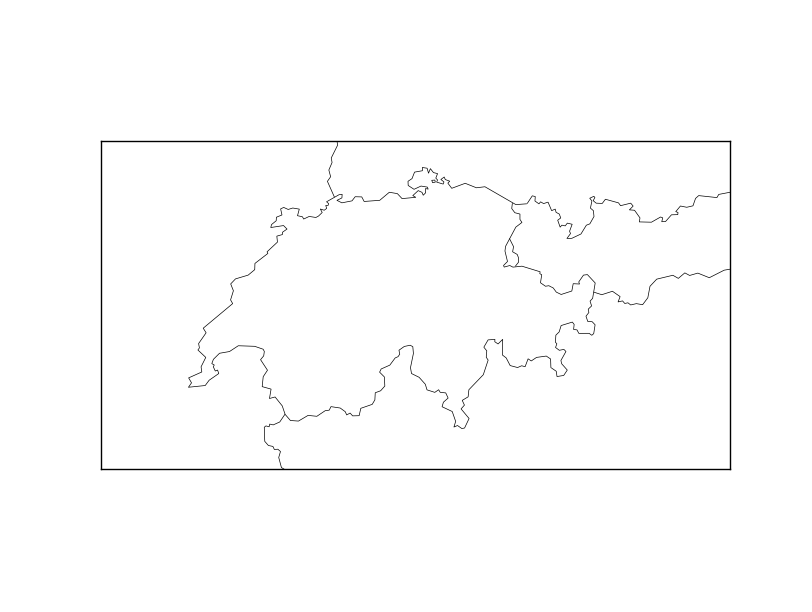
\includegraphics[width=0.8\textwidth]{pix/basemap_example_1}
\end{center}
\end{frame}

\begin{frame}[fragile]
\frametitle{Basemap}
\ldots adding a few details:
\begin{myColorBox}{1.0}{}
\begin{verbatim}
 >>> m.drawcoastlines()
 >>> m.drawcountries(linewidth=1.0)
 >>> m.drawmeridians([6,7,8,9,10,11],labels=[0,0,0,1])
 >>> m.drawparallels([46,46.5,47,47.5],labels=[1,0,0,0])
 >>> m.drawrivers(color='b')
 >>> x,y = m(8.540, 47.372)
 >>> m.scatter(x,y,c='r',marker='o')
 >>> plt.text(x,y,'Zurich',va='bottom')
 >>> plt.show()
\end{verbatim}
\end{myColorBox}
\pause
\begin{center}
      \includegraphics[width=0.7\textwidth]{pix/basemap_example_2_1}
\end{center}
\end{frame}

\begin{frame}[fragile]
\frametitle{Basemap}
Plot topography from the ETOPO1 global relief model:
\begin{myColorBox}{1.0}{}
\begin{verbatim}
>>> from scipy.io import netcdf
>>> from mpl_toolkits.basemap import Basemap, cm
>>> m = Basemap(projection='merc', llcrnrlat= 0, 
urcrnrlat=50, llcrnrlon=-80, urcrnrlon=50, lat_ts= 25, 
resolution='i')
>>> nc=netcdf.netcdf_file('ETOPO1_Ice_g_gmt4.grd')
>>> lons = nc.variables['x'].data
>>> lats = nc.variables['y'].data
>>> topoin = nc.variables['z'].data
>>> nx = int((m.xmax-m.xmin)/5000.)+1; 
>>> ny = int((m.ymax-m.ymin)/5000.)+1
>>> topodat = m.transform_scalar(topoin,lons,lats,nx,ny)
>>> im = m.imshow(topodat,cm.GMT_haxby)
>>> m.drawparallels(np.arange(0,50,20),labels=[1,0,0,0])
>>> m.drawmeridians(np.arange(-80,50,20),labels=[0,0,0,1])
>>> plt.show()
\end{verbatim}
\end{myColorBox}
\end{frame}

\begin{frame}[fragile]
\frametitle{Basemap}
\begin{center}
      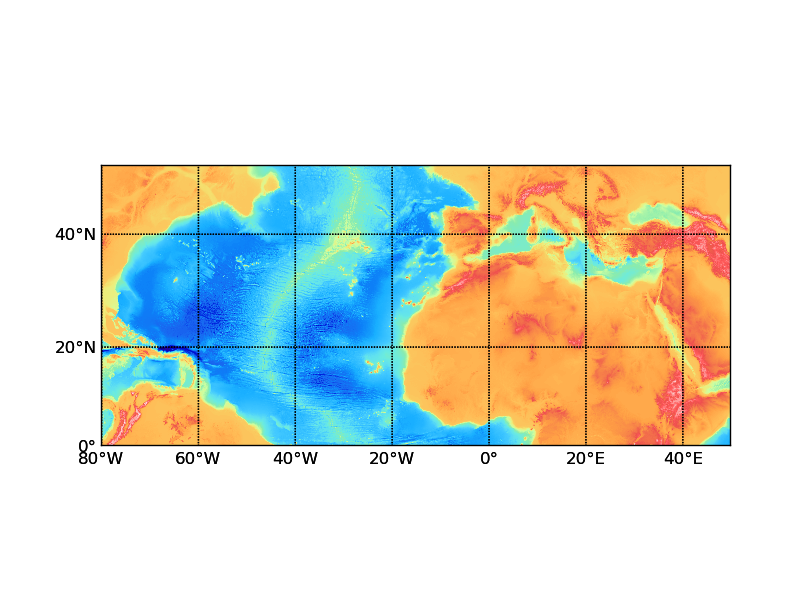
\includegraphics[width=1.0\textwidth]{pix/basemap_example_3}
\end{center}
\end{frame}

\begin{frame}[fragile]
\frametitle{Basemap}
Plot information from shapefile 
data from https://explore.data.gov/d/db3a-9tgn.
\begin{myColorBox}{0.9}{}
\begin{verbatim}
>>> m = Basemap(projection='mill',
llcrnrlon=-180. ,llcrnrlat=-60,
urcrnrlon=180. ,urcrnrlat=80.)
# assumes 'copper.shp', 'copper.shx' and 'copper.dbf'
# are in the current working directory 
>>> s = m.readshapefile('copper', 'copper')
>>> x, y = zip(*m.copper)
>>> m.drawcoastlines()
>>> m.fillcontinents()
>>> plt.plot(x, y, 'b.')
>>> plt.title('World copper smelters locations')
>>> plt.show()
\end{verbatim}
\end{myColorBox}
\end{frame}

\begin{frame}[fragile]
\frametitle{Basemap}
\begin{center}
      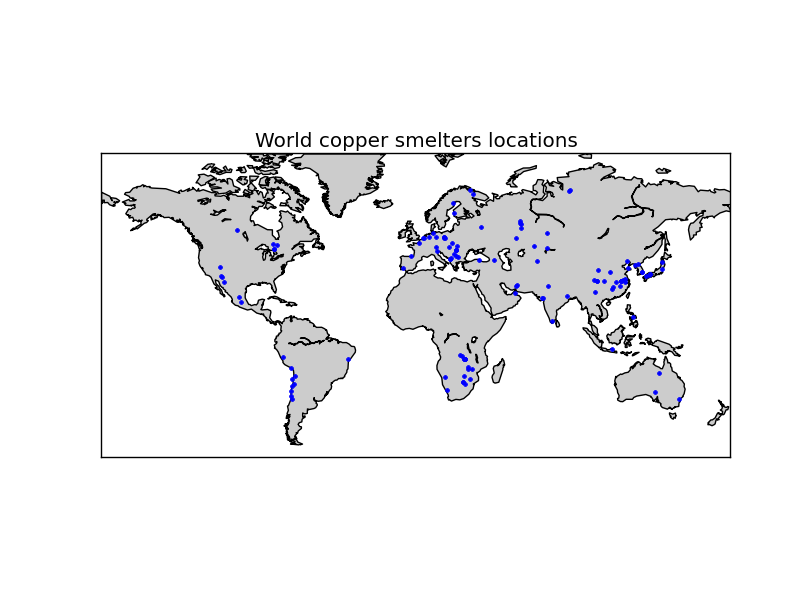
\includegraphics[width=1.0\textwidth]{pix/basemap_example_4}
\end{center}
\end{frame}

\begin{frame}
\begin{center}
\Huge{pyproj}
\end{center}
\end{frame}

\begin{frame}[fragile]
\frametitle{pyproj}
\begin{itemize}
  \item Pyproj provides python bindings to the PROJ4 library.
  \item Convert from geographic (longitude,latitude)
	to native map projection (x,y) coordinates and vice versa
   \item Convert from one map projection coordinate system directly to another
   \item Perform great circle computations such as determining distance, azimuth
   and back-azimuth between two given points
\end{itemize}

Convert longitude and latitude of Zurich into UTM coordinates and back:
 \begin{myColorBox}{0.9}{}
\begin{verbatim}
>>> p = pyproj.Proj(proj="utm",zone=32)
>>> p(8.540, 47.372)
(465271.7360602605, 5246607.042608537)
>>> p(*(_),inverse=True)
(8.54, 47.371999999999986)
\end{verbatim}
\end{myColorBox}
\end{frame}

\begin{frame}[fragile]
\frametitle{pyproj}
Great circle computation: compute azimuth, back-azimuth and distance between
Zurich and Basel and do the inverse.
\begin{myColorBox}{1.0}{}
\begin{verbatim}
>>> g = pyproj.Geod(ellps='WGS84')
>>> az, baz, dist = g.inv(8.540, 47.372, 7.593, 47.560)
>>> az, baz, dist
(-73.33366215015755, 105.9685077646491, 74392.53849627372)
>>> lon, lat, baz = g.fwd(8.540, 47.372, az, dist)
>>> lon,lat,baz
(7.592999999296916, 47.56000000001562, 105.96850776458967)
\end{verbatim}
\end{myColorBox}
\end{frame}

\begin{frame}
\begin{center}
\Huge{Exercises}
\end{center}
\end{frame}

